\newpage
\section{Конструкторская часть}

В данной работе для нахождения расстояния Левенштейна используется матричный
алгоритм, а для Дамерау-Левенштейна матричный и рекурсивный. Далее будут
рассмотрены все эти алгоритмы.

\subsection{Функциональная модель}

На рисунке 1 представлена IDEF0.

\begin{center}
    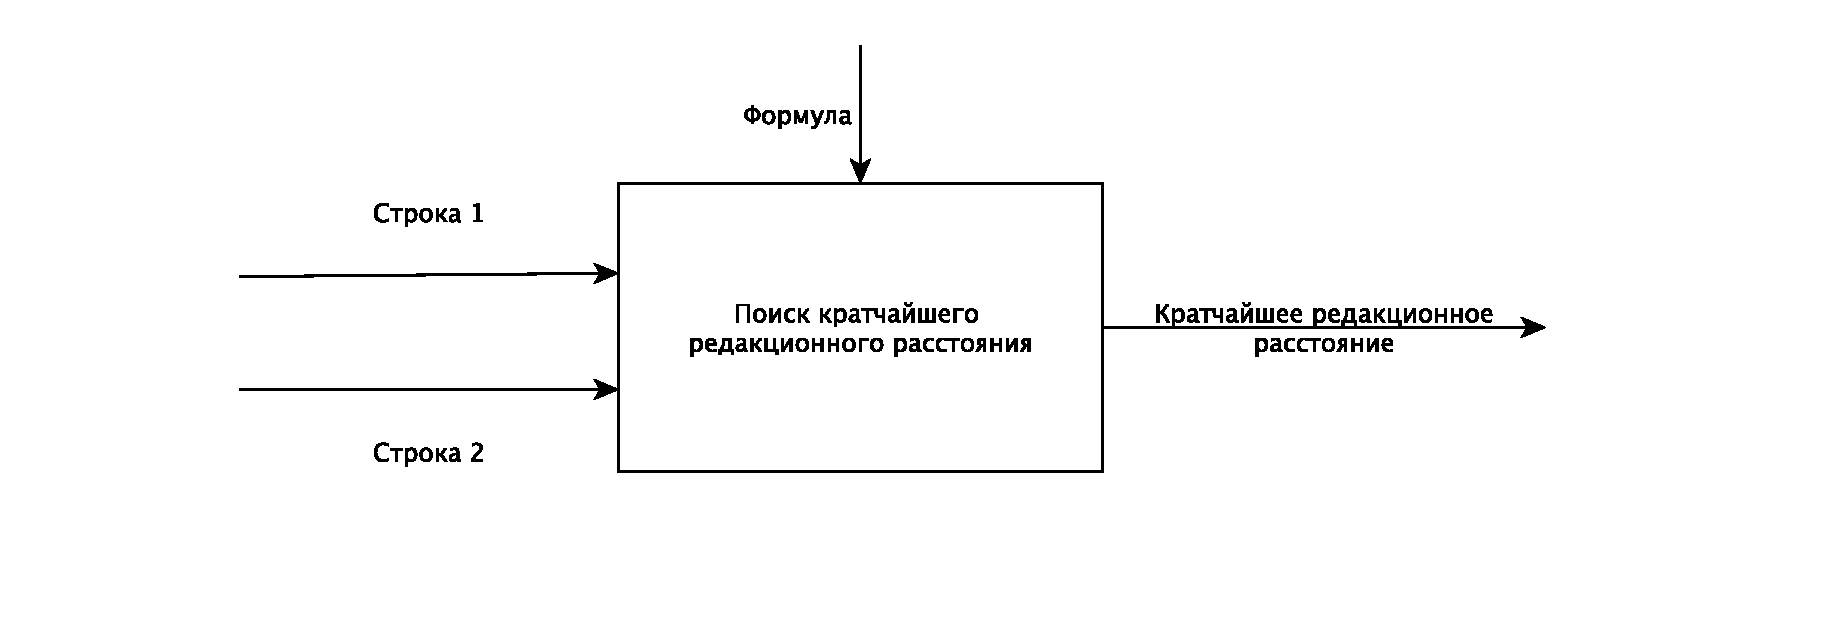
\includegraphics[scale=0.5]{IDEF0}

    Рисунок 1. IDEF0
\end{center}

\subsection{Схемы алгоритмов}

На рисунке 2 представлена схема матричного алгоритма расчета расстояния Левенштейна.

\begin{center}
    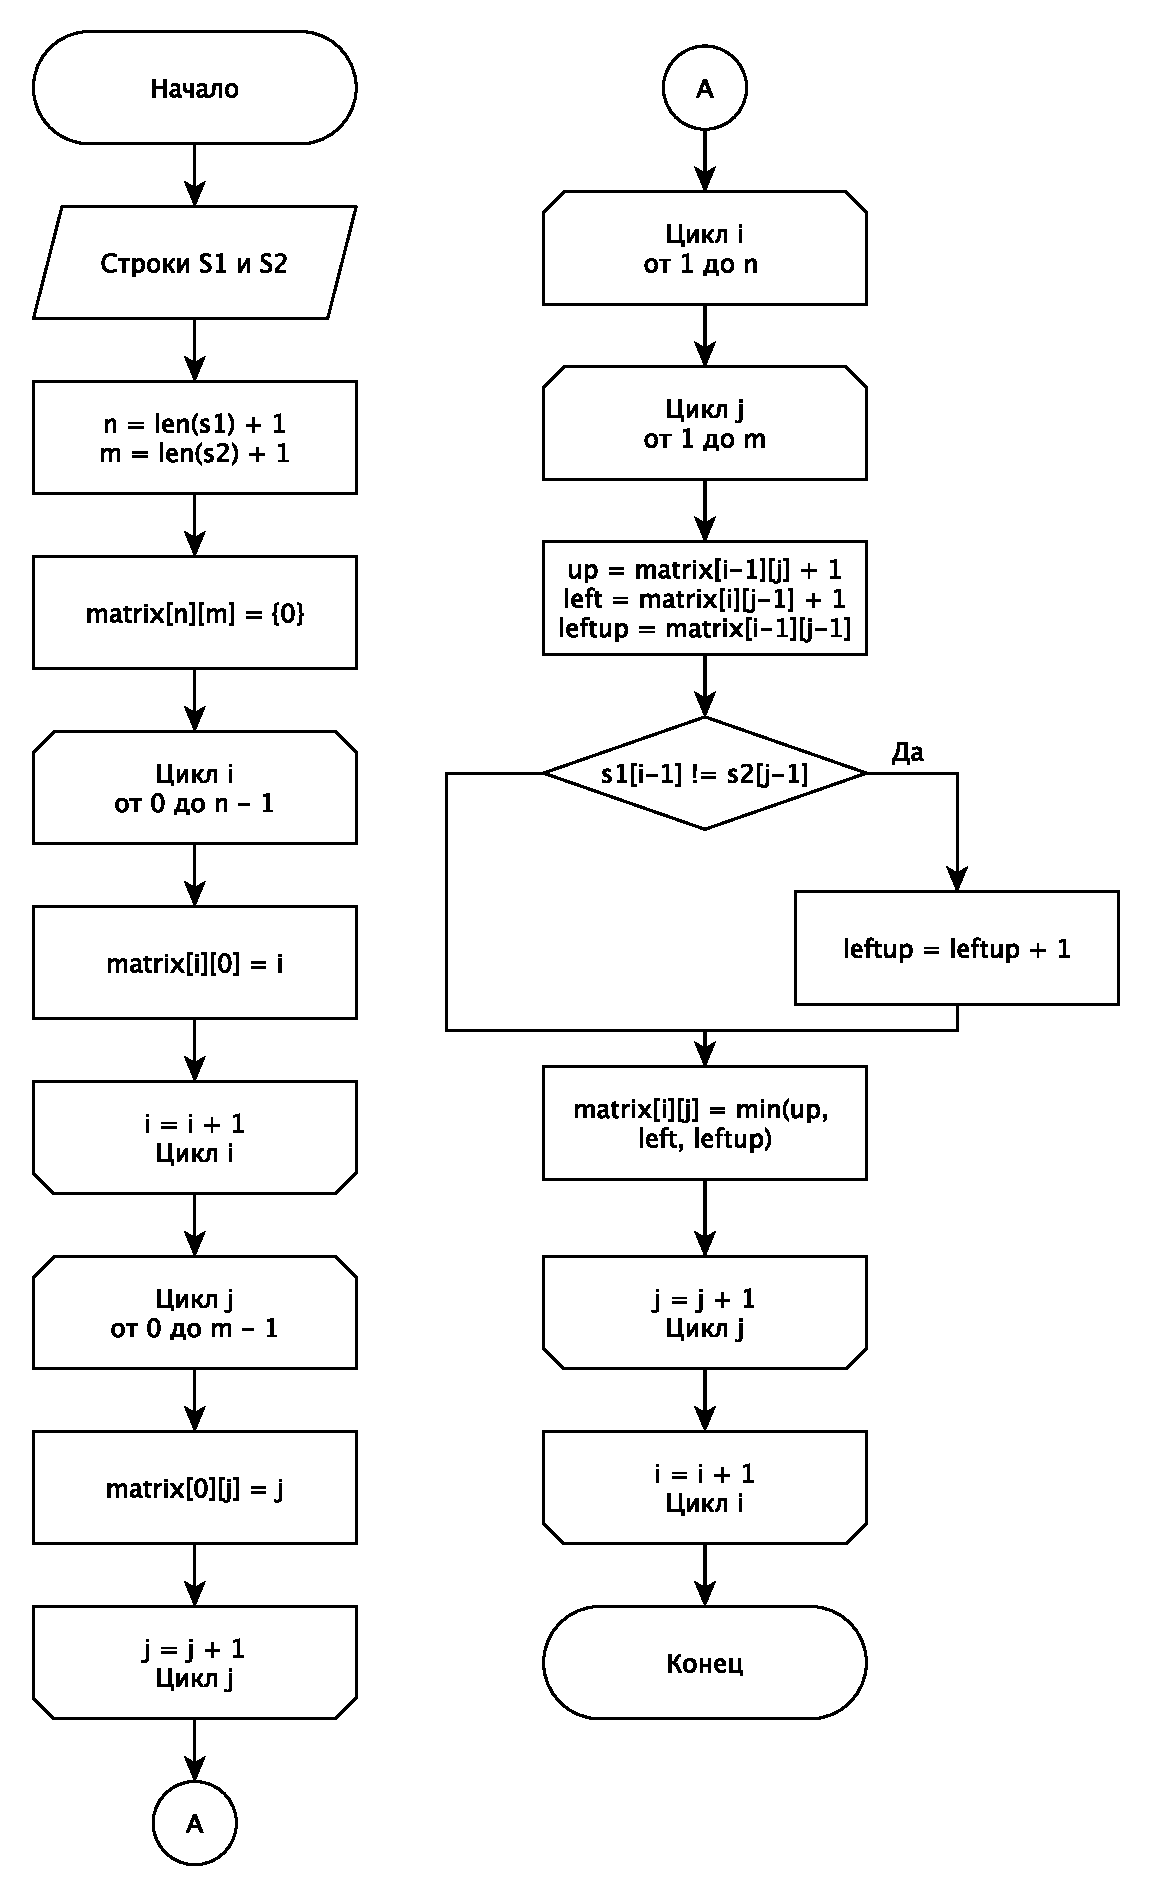
\includegraphics[scale=0.7]{Lmatrix}

    Рисунок 2. Матричный алгоритм расчета расстояния Левенштейна
\end{center}

На рисунке 3 представлена схема матричного алгоритма расчета расстояния Дамерау-Левенштейна.

\begin{center}
    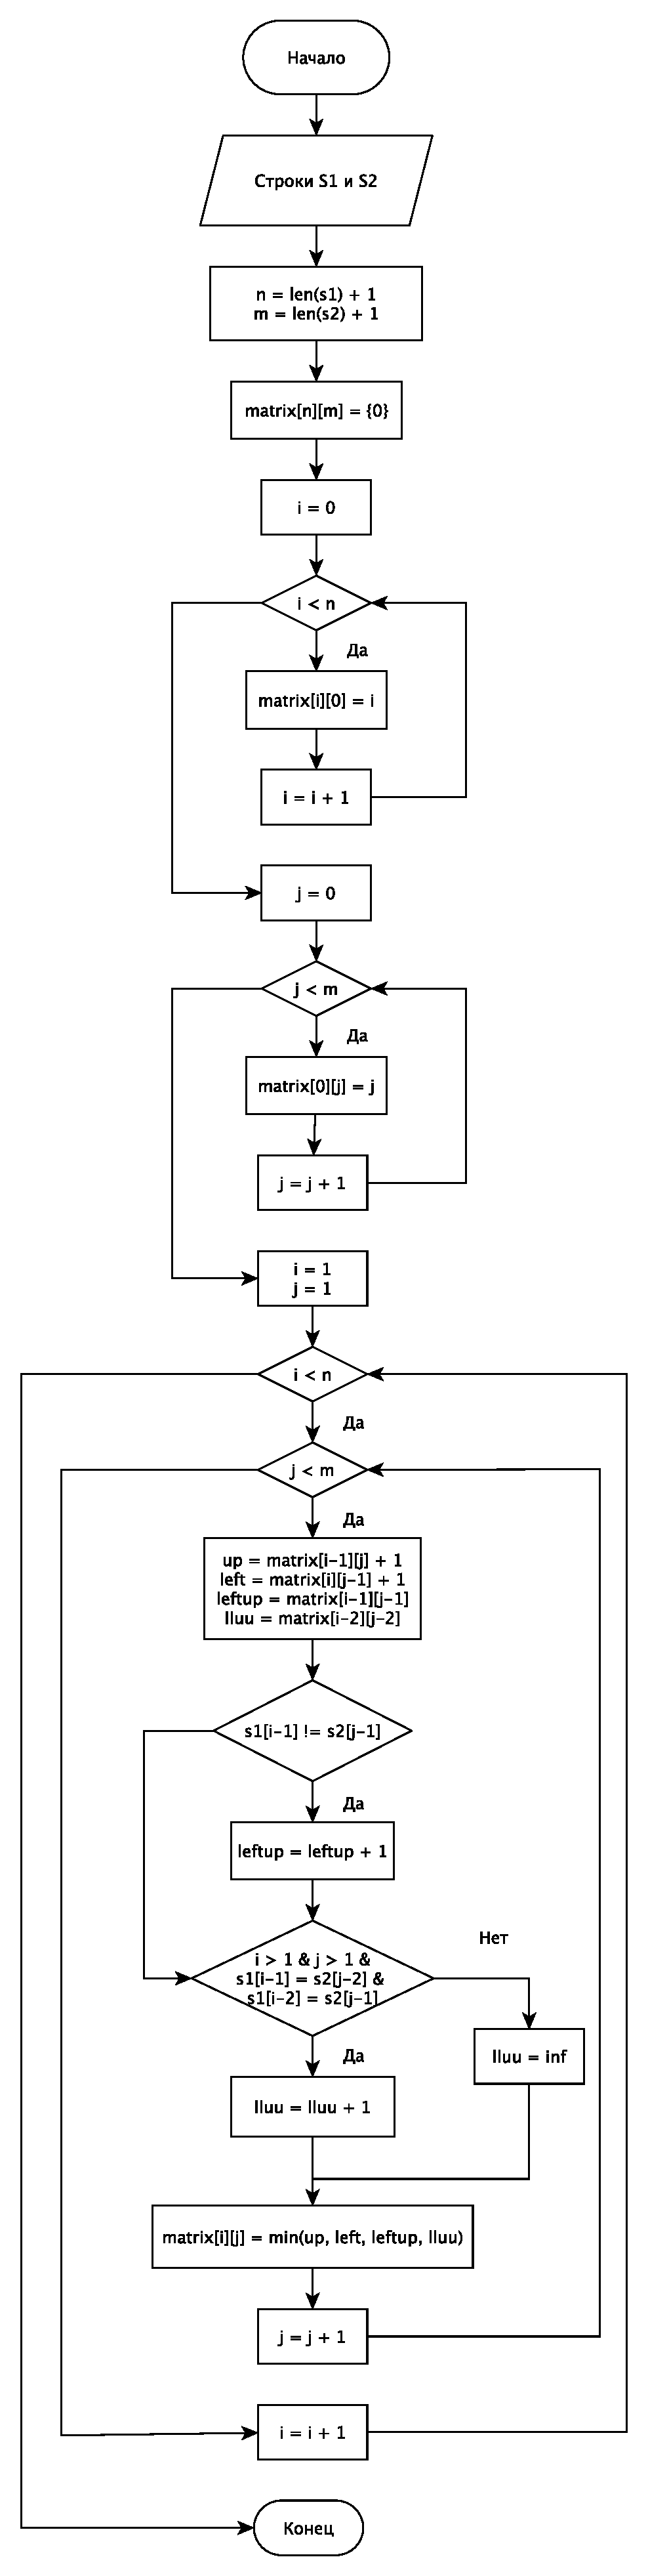
\includegraphics[scale=0.6]{DLmatrix}

    Рисунок 3. Матричный алгоритм расчета расстояния Дамерау-Левенштейна
\end{center}

На рисунке 4 представлена схема рекурсивного алгоритма расчета расстояния Дамерау-Левенштейна.

\begin{center}
    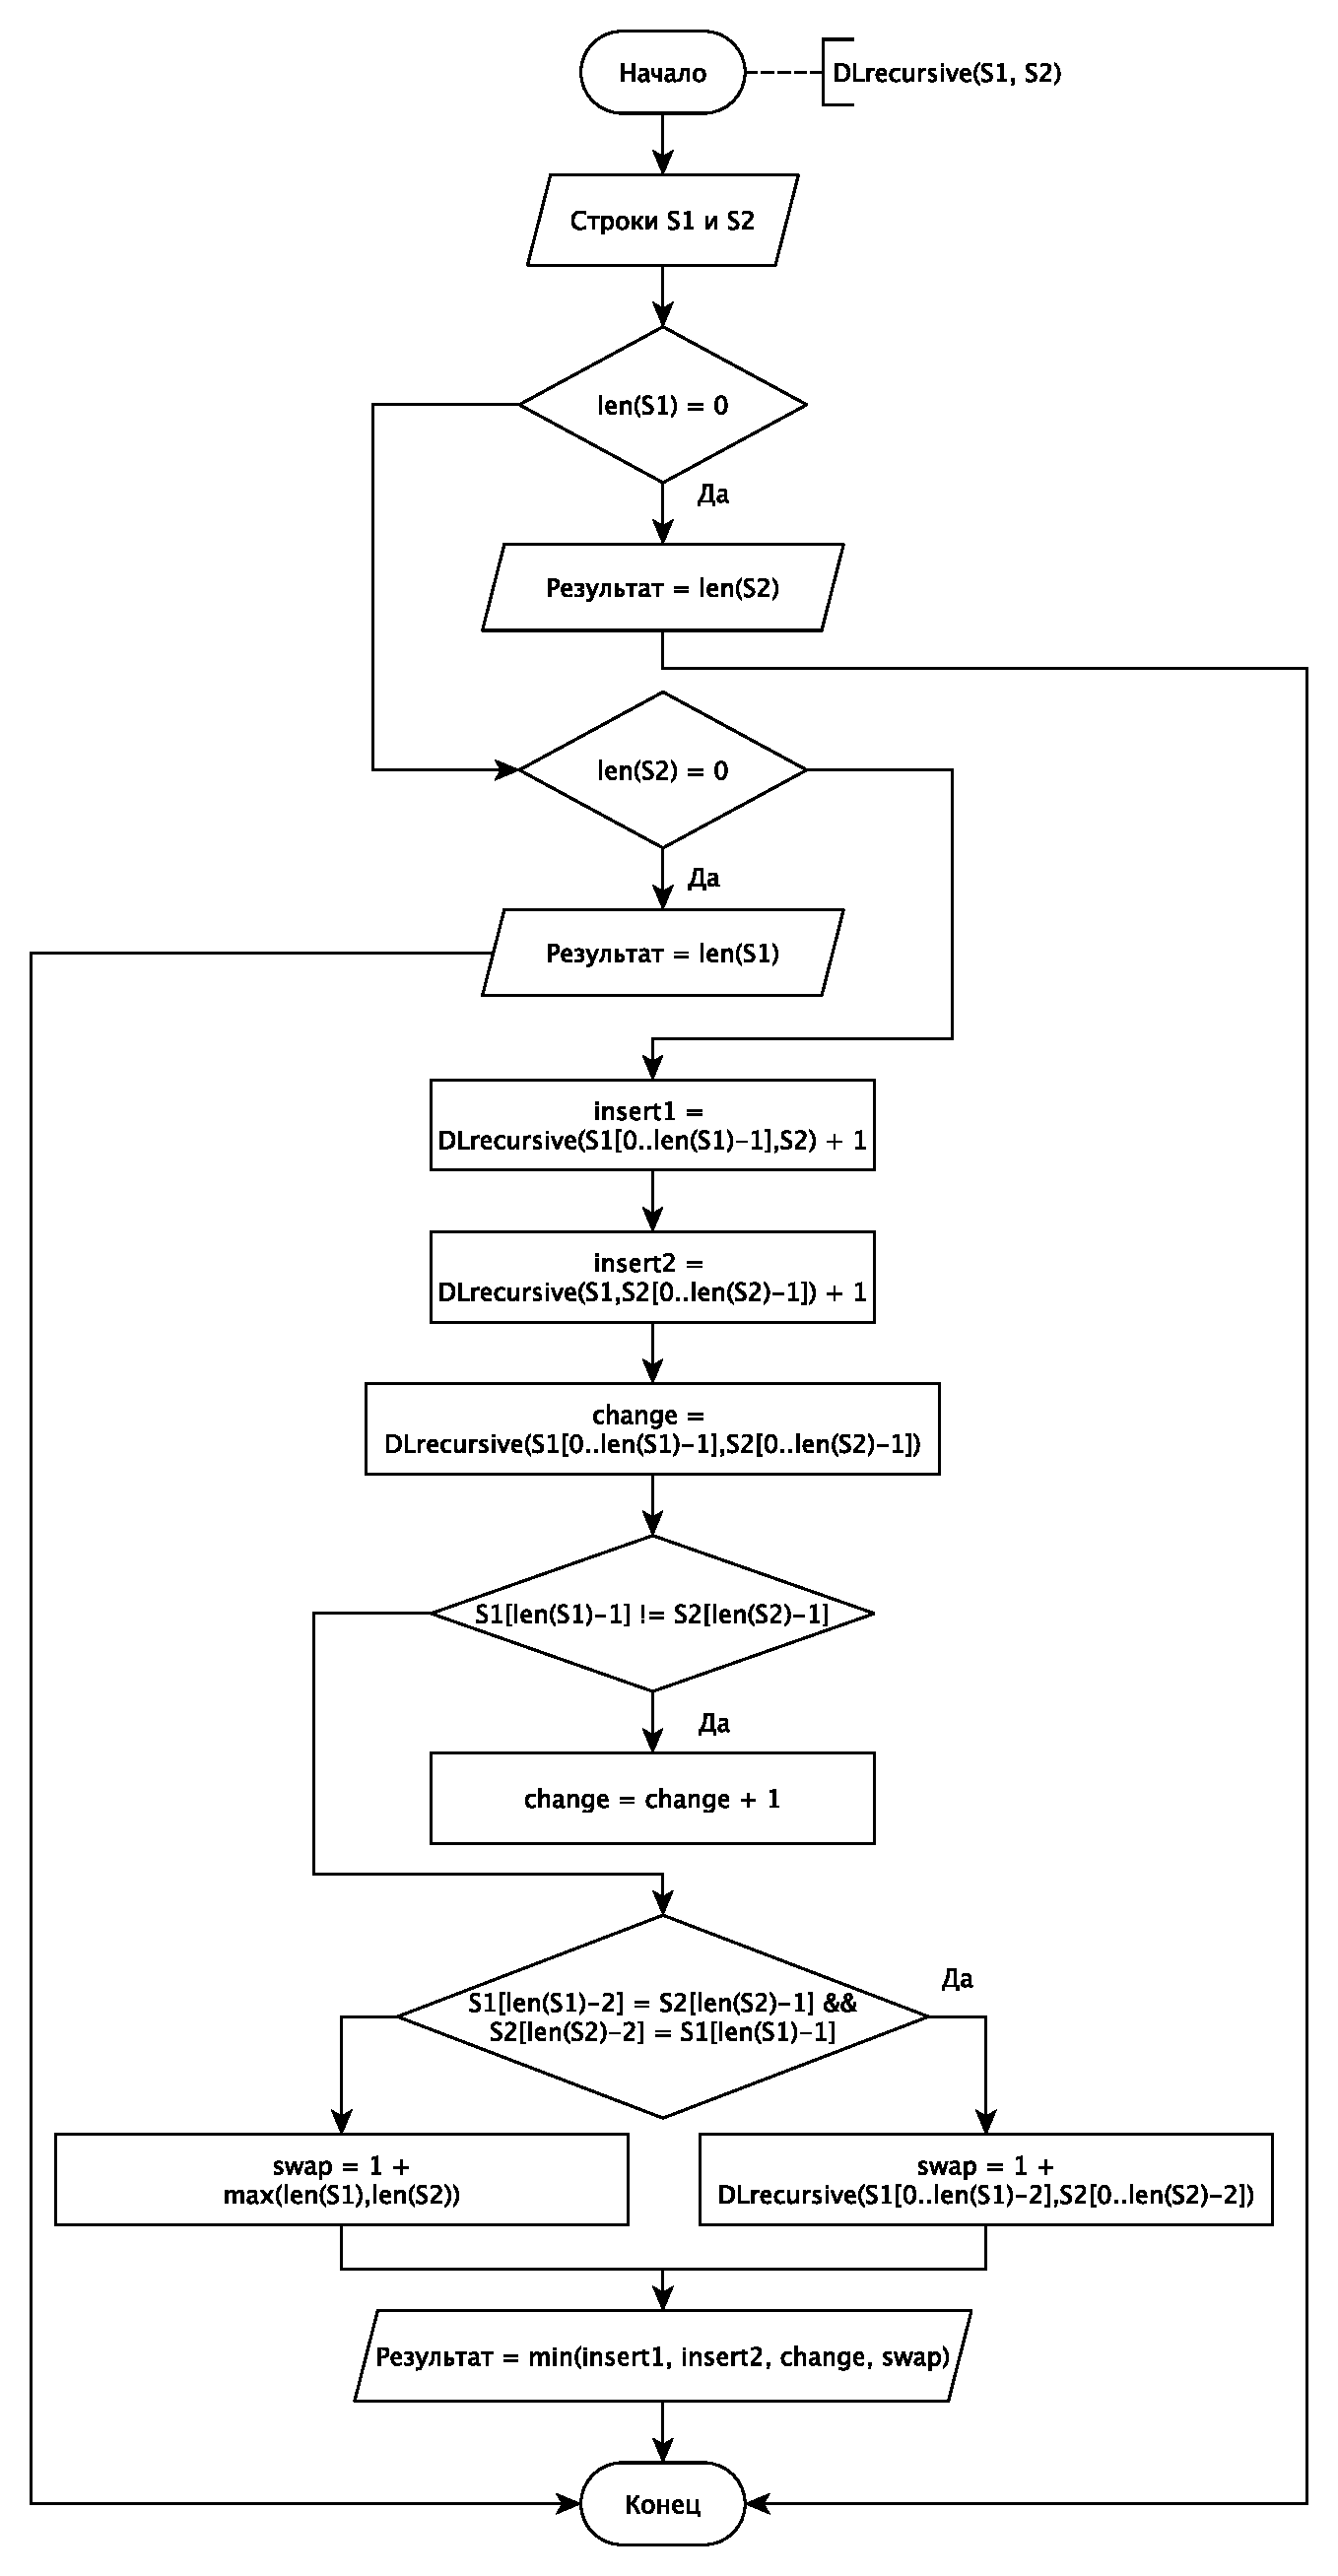
\includegraphics[scale=0.4]{DLrecursive}

    Рисунок 4. Рекурсивный алгоритм расчета расстояния Дамерау-Левенштейна
\end{center}

\subsection{Выводы}

Рекурсивный алгоритм имеет сложность $\Omega (4^{max(n,m)})$, а матричные
$\Omega (n \cdot m)$. Таким образом очевидно, что рекурсивный алгоритм
сильно проигрывает матричным по времени. Проверим данное предположение
на реализованных алгоритмах.
